
\section{Machine Learning}
\label{sec:background:ml}

Machine Learning (ML) is a branch of AI focusing on improving the automatic
learning of models without having been explicitly programmed for it. ML comes
with three basic paradigms: supervised, unsupervised, and reinforcement
learning. Each of them is defined below.

\begin{multicols}{2}
  \begin{definition}[Supervised Learning]
    Type of ML with human supervision, where a model looks for patterns in a data
    set with labels~\citep{website:deepai:unsupervised:learning}.
    \label{def:supervised:learning}
  \end{definition}

  \begin{definition}[Unsupervised Learning]
    Type of ML with minimal human supervision, where a model looks for patterns
    in a data set without labels.
    \label{def:unsupervised:learning}
  \end{definition}
\end{multicols}

Visually, supervised learning and unsupervised learning are defined as follows:
\begin{figure}[!ht]
  \centering
  \begin{minipage}{.45\textwidth}
    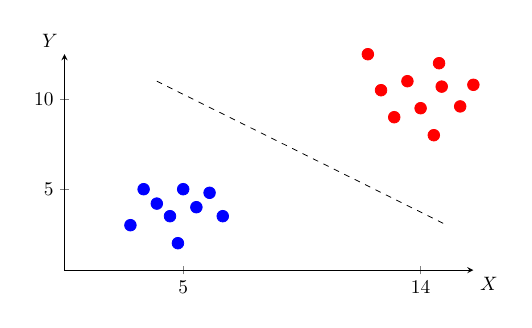
\begin{tikzpicture}[baseline,scale=.7]
      \begin{axis}[
        height=5.5cm,
        width=9cm,
        axis x line=center,
        axis y line=center,
        xlabel style={below right},
        ylabel style={above left},
        xlabel={$X$},
        ylabel={$Y$},
        xtick={4,10},
        xtick={5,14},
        clip mode=individual
        ]

        % Trick to display the graph starting at (1,1)
        \addplot[green,mark size=0] table [%
        x = x,
        y = y,
        col sep = comma]{
          x,y
          0.5,0.5
        };

        \addplot[blue, only marks, mark=*, mark size=3] table [%
        x = x,
        y = y,
        col sep = comma]{
          x,y
          3,3
          3.5,5
          4,4.2
          4.5,3.5
          4.8,2
          5,5
          5.5,4
          6,4.8
          6.5,3.5
        };

        \draw [dashed] (4,11) -- (15,3);

        \addplot[red, only marks, mark=*, mark size=3] table [%
        x = x,
        y = y,
        col sep = comma]{
          x, y
          12,12.5
          12.5,10.5
          13,9
          13.5,11
          14,9.5
          14.5,8
          14.7,12
          14.8,10.7
          15.5,9.6
          16,10.8
        };
      \end{axis}
    \end{tikzpicture}
    \captionof{figure}{Supervised Learning}
    \label{tikz:background:supervised:learning}
  \end{minipage}
  \quad
  \begin{minipage}{.45\textwidth}
    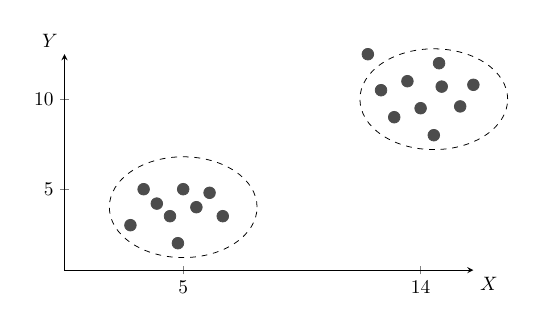
\begin{tikzpicture}[baseline,scale=.7]
      \begin{axis}[
        height=5.5cm,
        width=9cm,
        axis x line=center,
        axis y line=center,
        xlabel style={below right},
        ylabel style={above left},
        xlabel={$X$},
        ylabel={$Y$},
        xtick={4,10},
        xtick={5,14},
        clip mode=individual
        ]

        % Trick to display the graph starting at (1,1)
        \addplot[mark size=0] table [%
        x = x,
        y = y,
        col sep = comma]{
          x,y
          0.5,0.5
        };

        \addplot[black!70,only marks, mark=*, mark size=3] table [%
        x = x,
        y = y,
        col sep = comma]{
          x,y
          3,3
          3.5,5
          4,4.2
          4.5,3.5
          4.8,2
          5,5
          5.5,4
          6,4.8
          6.5,3.5
        };

        \draw [dashed] (5,4) circle[radius=2.8];

        \addplot[black!70,only marks, mark=*, mark size=3] table [%
        x = x,
        y = y,
        col sep = comma]{
          x, y
          12,12.5
          12.5,10.5
          13,9
          13.5,11
          14,9.5
          14.5,8
          14.7,12
          14.8,10.7
          15.5,9.6
          16,10.8
        };
        \draw [dashed] (14.5,10) circle[radius=2.8];
      \end{axis}
    \end{tikzpicture}
    \captionof{figure}{Unsupervised Learning}
    \label{tikz:background:unsupervised:learning}
  \end{minipage}
  \caption{Learning a Model Using Raspberry and Blueberry Data.}
  \label{fig:background:supervised:vs:unsupervised}
\end{figure}

In Figure \ref{tikz:background:supervised:learning}, supervised learning
contains raspberry and blueberry data already classified by their label. A model
learns to predict the values based on a \emph{cost function}, which allows it to
check and correct its predictions according to the actual values. With these
labeled data, the classification and regression problems can use this type of
learning.

In Figure \ref{tikz:background:unsupervised:learning}, unsupervised learning
still contains raspberry and blueberry data. However, this time these data are
not labeled, which means that a model must find the patterns and structure
independently. The clustering and association problems use this type of
learning. For example, this clustering example creates two clusters, with one
raspberry not belonging to any cluster.


\begin{definition}[Reinforcement Learning]
  Type of ML where a model learns from the experience and feedback of an
  autonomous agent.
\end{definition}

\noindent In ML, each neuron inside an Artificial Neural Networks (ANN) outputs
a number between $-\infty$ and $\infty$ propagating to its predecessor via an
activation function. Once the ANN has completed its processing through these
neurons, it generates \emph{logits}, a non-normalized vector of predictions
generated by a classification model. For ease of processing, it is usually
appropriate to convert these logits into probabilities to have a unitary
sum. According to the required type of classification, activation functions such
as \emph{softmax} and \emph{sigmoid} are helpful. These functions can help with
various tasks, such as predicting the most likely word to be the missing word in
a sentence in the Natural Language Processing (NLP) field.

\begin{definition}[Softmax Function]
  Also called \emph{softargmax}, a logistic regression model uses this
  multi-classification function for transformation purposes. Specifically, this
  model transforms a vector of $K$ real values into a vector of $K$ elements that
  range between 0 and 1 with the particularity of having a unitary
  sum~\citep{website:deepai:softmax}. Let $\mathbf{z}$ be an input vector and $K$
  be some classes in a multi-class classifier. Mathematically, the softmax
  function of these classes is defined as follows:
  \begin{equation}
    \mathrm{\sigma}(\mathbf{z})_i = \frac{\me^{z_i}}{\sum^K_{j=1}\me^{z_j}}
    \label{eq:softmax}
  \end{equation}
  \label{def:softmax}
\end{definition}

\begin{definition}[Sigmoid Function]
  Binary classification function recognizable with an ``S'' shaped curve used by
  a logistic regression model for transformation purposes. Unlike the softmax
  function, this model transforms a vector of $K$ real values into a vector of $K$
  elements range this time between -1 and 1 with still the particularity of having
  a unitary sum. Let $\mathbf{x}$ be an input vector. Mathematically, the
  sigmoid function is defined as follows:
  \begin{equation}
    \mathrm{\sigma}(\mathbf{x}) = \frac{1}{1 + e^{-x}} = \frac{e^x}{e^x + 1}
    \label{eq:sigmoid}
  \end{equation}
  \label{def:sigmoid}
\end{definition}

\begin{definition}[Rectified Linear Unit]
  Commonly called \emph{ReLU}, the community considers this function as one of
  the most straightforward functions. Let $\mathbf{x}$ be an input
  vector. Mathematically, the ReLU function is defined as follows:
  \begin{equation}
    \mathrm{f}(\mathbf{x}) = \max(0, \mathbf{x})
    \label{eq:relu}
  \end{equation}
  \label{def:relu}
\end{definition}

\noindent These functions can help with various tasks, such as predicting the
most likely word to be the missing word in a sentence in the NLP
field. Subsequently, in ML, it is essential to know the similarity of two
vectors. For example, it is helpful in NLP to tell if two words share semantic
similarities. As a result, the use of cosine similarity is relevant.

\begin{definition}[Cosine Similarity]
  Measures the cosine of the angle between two non-zero vectors of an inner
  product space~\citep{website:deepai:cosine:similarity}. Let $\mathbf{u},
  \mathbf{v} \in \mathbb{R}^d$ be two non-zero $d$-dimensional vectors.
  Mathematically, the cosine similarity between $\mathbf{u}$ and $\mathbf{v}$ is
  defined as follows:
  \begin{align}
    \cos(\mathbf{u}, \mathbf{v}) =
    \frac{\mathbf{u} \cdot \mathbf{v}}
    {\left\lVert \mathbf{u} \right\rVert
    \left\lVert \mathbf{v} \right\rVert} =
    \frac{\sum\limits_{i = 1}^n u_i v_i}
    {\sqrt{\sum\limits_{i = 1}^n u_i^2}
    \sqrt{\sum\limits_{i = 1}^n v_i^2}}
    \label{eq:cosine:similarity}
  \end{align}

  where $\cos(\mathbf{u}, \mathbf{v})$ produces a value ranging from -1 to 1.
  Specifically, the cosine similarity returns -1 if two vectors do not have any
  similarities, 0 if they are unrelated, and 1 if they share every similarity.
  \label{def:cosine:similarity}
\end{definition}

%%% Local Variables:
%%% mode: latex
%%% TeX-master: "../../report"
%%% End:
